\documentclass[a4paper]{article}

\usepackage[utf8]{inputenc}
\usepackage[ngerman]{babel}
\usepackage[T1]{fontenc}
\usepackage{listings}
\usepackage{hyperref}
\usepackage{graphicx}
\usepackage{gensymb}
\usepackage{float}

\lstset{basicstyle=\ttfamily,columns=fullflexible}
\lstset{literate=%
	{Ö}{{\"O}}1
	{Ä}{{\"A}}1
	{Ü}{{\"U}}1
	{ß}{{\ss}}1
	{ü}{{\"u}}1
	{ä}{{\"a}}1
	{ö}{{\"o}}1
}
\newcommand*{\thead}[1]{\multicolumn{1}{c}{\bfseries #1}}

\begin{document}

\title{Heizungssteuerung}
\author{Viktor Saibel \& Daniel Tkocz}
\maketitle

\newpage

\tableofcontents

\newpage

\section{Einleitung}
Ziel des Projekts ist die Temperaturregelung mit einem Stellventil und einem Temperatursensor mittels KNX- und EnOcean-Kommunikationstechnologien.
Es soll erreicht werden, dass der Temperatursensor die Raumtemperatur misst und diese dem Stellwerk mitteilt. Dieses muss die übermittelte Temperatur nutzen um das Ventil so zu steuern, dass eine definierte Zieltemperatur im Raum herrscht.

\section{Hardware}
\subsection{SIEMENS 5WG1220-2AB21 Tasterschnittstelle UP220/21}
Bei dem Gerät handelt es sich um eine Schnittstelle für einen Taster sowie eine LED. Der Taster kann in diversen Modi betrieben werden und die LED ist unabhängig von dem Taster verwendbar.
Für weiter Informationen zu dem Produkt kann man auf der \href{http://www.buildingtechnologies.siemens.com/bt/global/de/products/Gamma-Geb%C3%A4udesystemtechnik/Gamma-instabus---KNX/Eingabeger%C3%A4te/Seiten/UP%20220_221.aspx}{Herstellerseite} nachsehen.
	\subsection{Thermokon SAB05 Ventilstellantrieb}
	Das Gerät ist ein per Funk gesteuerter Ventilstellantrieb.
	Die Kommunikation und Konfiguration erfolgt über das EnOcean Protokoll.
	Zudem verfügt das Gerät über einen Temperatursensor.
	Entgegen dem Konzept von EnOcean verwendet das Gerät drei AA-Batterien.
	Eine Konfiguration ist mittels AirConfig (Thermokon Programm) sowie eingeschränkt per Tastendruck und LED-Status möglich.
	Für weiter Informationen zu dem Produkt kann man auf der \href{https://www.thermokon.de/en/products/easysensr-receiver/actuators/sab05/}{Herstellerseite} nachsehen.
	\subsection{Weinzierl KNX ENO 634 Bidirektionales Gateway}
	Das Gerät ist ein Gateway zur Kommunikation mit EnOcean Geräten über die KNX-Technologie. Das Gateway kümmert sich um sämtliche Kommunikation mit den EnOcean-Geräten. Die EnOcean-Geräte werden nicht als solche in der ETS konfiguriert. Stattdessen wird in dem Gateway ein Gerät von dem gewünschten Typ (z.B. Ventilstellantrieb) angelegt und konfiguriert. Dazu kann einer von 32 Funkkanälen gewählt werden. Somit muss man mehrere Gateways verwenden, möchte man mehr als 32 EnOcean-Geräte benutzen.
	Für weiter Informationen zu dem Produkt kann man auf der \href{https://www.weinzierl.de/index.php/de/alles-knx1/knx-devices/knx-eno-634}{Herstellerseite} nachsehen.

\section{Umsetzung}
\subsection{Grundlagen}
Nach dem Herunterladen und Installieren der Software ETS5 von \href{https://www.knx.org/knx-de/software/ets/herunterladen/index.php}{knx.org} muss ein neues Projekt angelegt werden. Dies ist in Abbildung \ref{fig:1} zu sehen.

\begin{figure}[H]
\centering
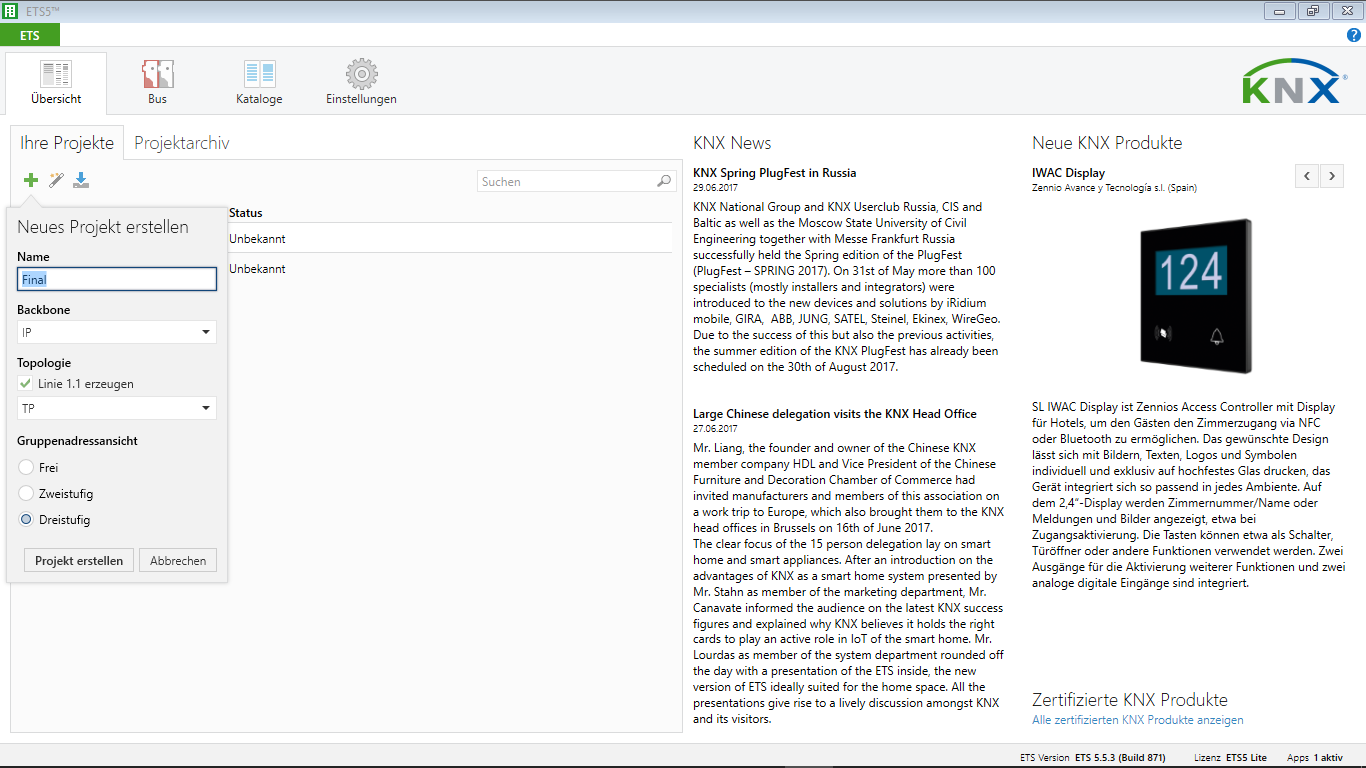
\includegraphics[width=13cm]{Doku/1}
\caption{Erstellen eines ETS5 Projekts}
\label{fig:1}
\end{figure}

Damit Komponenten zu dem Projekt hinzugefügt werden können, muss in dem Projekt ein Gebäude erstellt werden. In Abbildung \ref{fig:2} wurde Beispielhaft das C-Gebäude angelegt.

\begin{figure}[H]
\centering
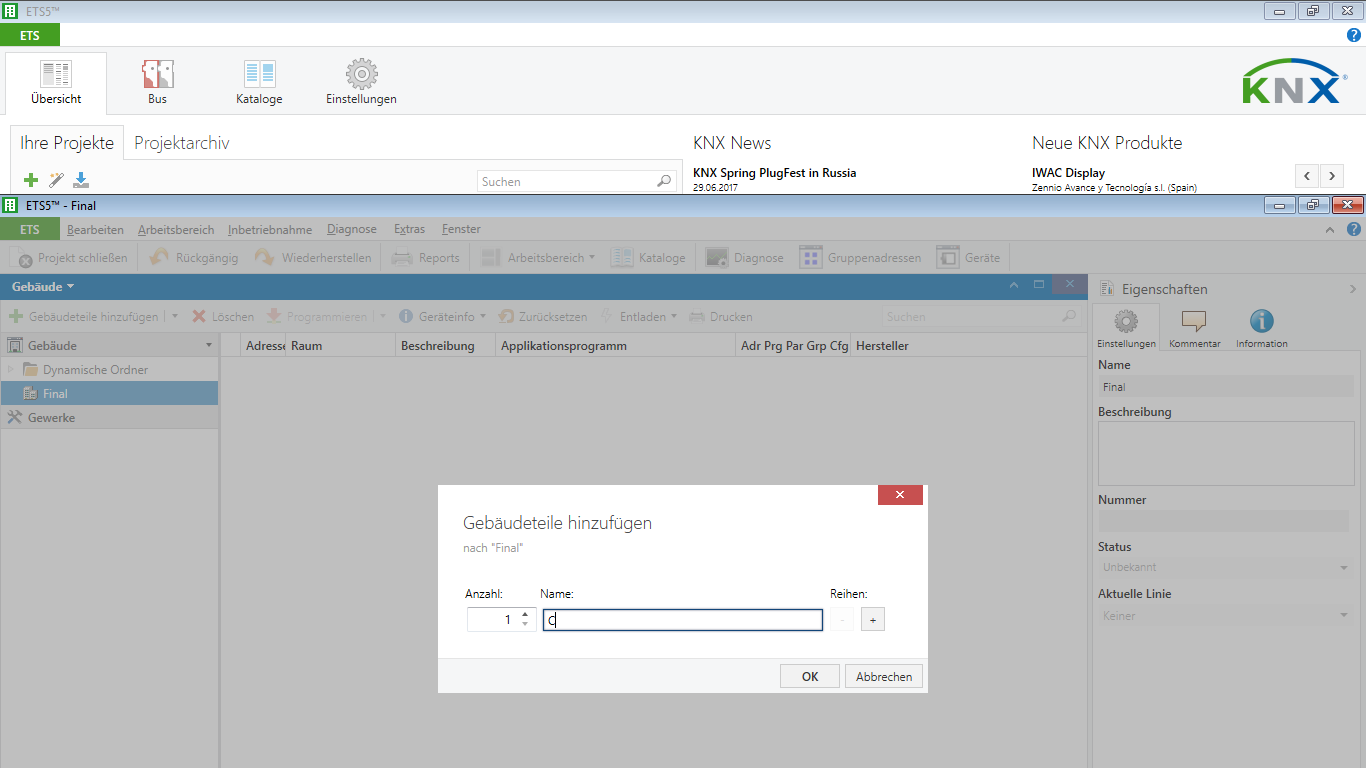
\includegraphics[width=13cm]{Doku/2}
\caption{Erstellen eines Gebäudes}
\label{fig:2}
\end{figure}

Ein Raum muss zusätzlich erstellt werden. Abbildung \ref{fig:3} zeigt wie Raum C031 angelegt wurde.

\begin{figure}[H]
\centering
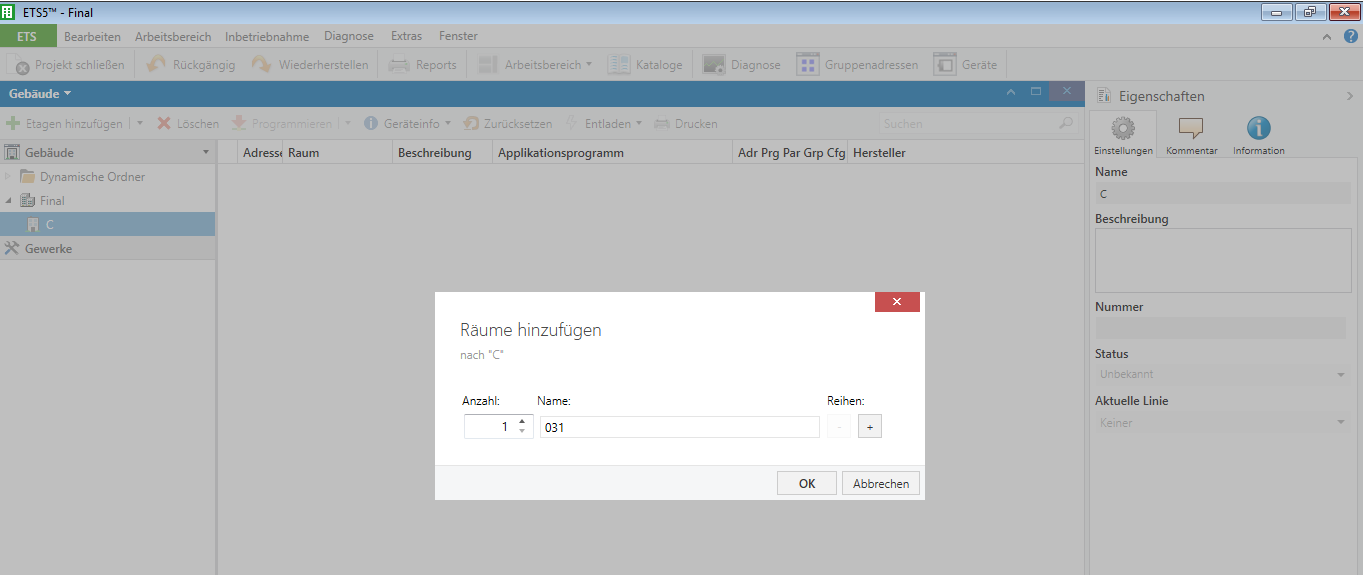
\includegraphics[width=13cm]{Doku/3}
\caption{Anlegen eines Raumes}
\label{fig:3}
\end{figure}

Sollen Geräte hinzugefügt werden, müssen von dem jeweiligen Hersteller die entsprechenden Konfigurationsdateien heruntergeladen werden und in ETS5 importiert werden. Dazu werden Administrationsrechte benötigt. Abbildung \ref{fig:4} zeigt Beispielhaft eine Auswahl an möglichen Geräten. Im Falle des vorhandenen Thermostats ist diese Datei unter \href{https://www.weinzierl.de/images/download/software_tools/Weinzierl_KNX_Eno_63x_Tool.zip}{www.weinzierl.de} zu finden. Auf diese Weise sind alle Geräte einzubinden, die man programmieren möchte.

\begin{figure}[H]
	\centering
	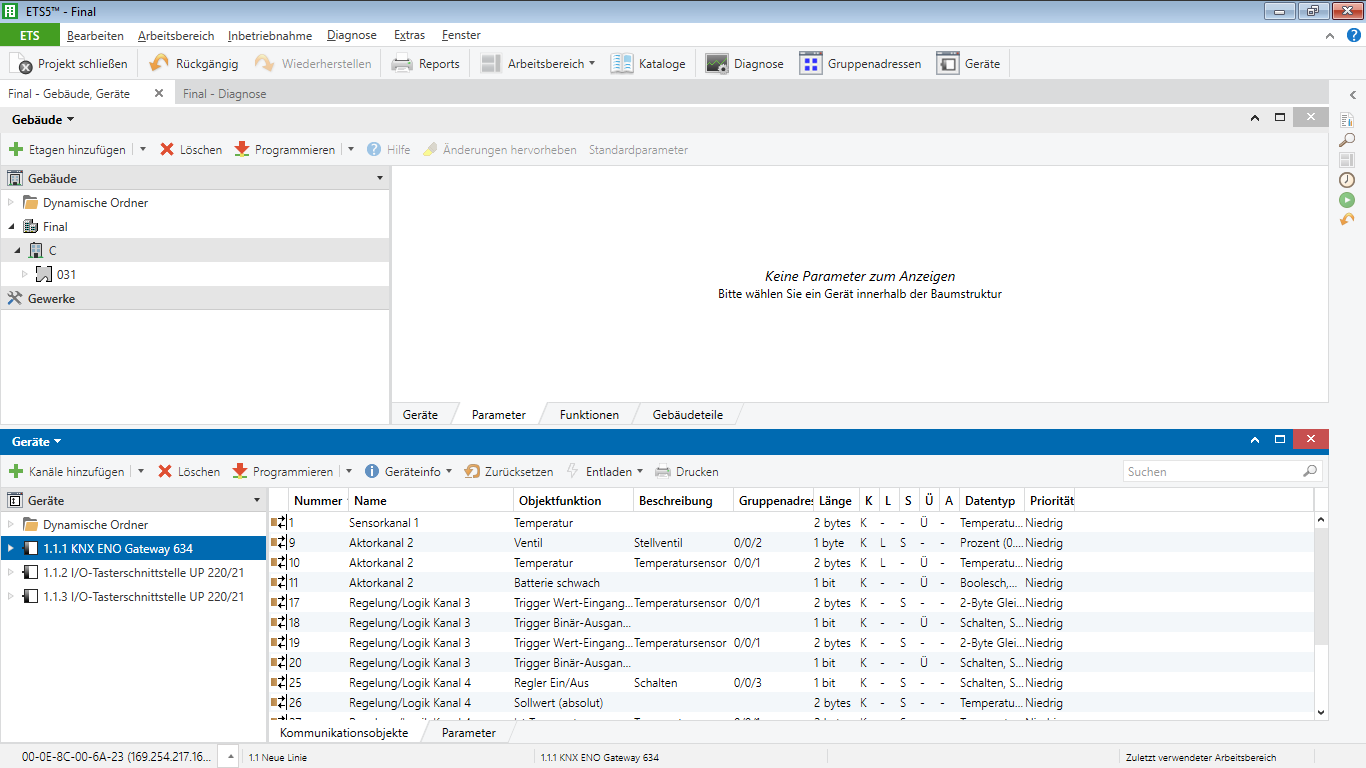
\includegraphics[width=13cm]{Doku/4}
	\caption{Übersicht der Gerätekonfigurationen}
	\label{fig:4}
\end{figure}

Per Drag \& Drop lassen sich diese Geräte in das Projekt importieren. Eine Auflistung aller Geräte des Projekts wird in Abbildung \ref{fig:5} gezeigt.

\begin{figure}[H]
	\centering
	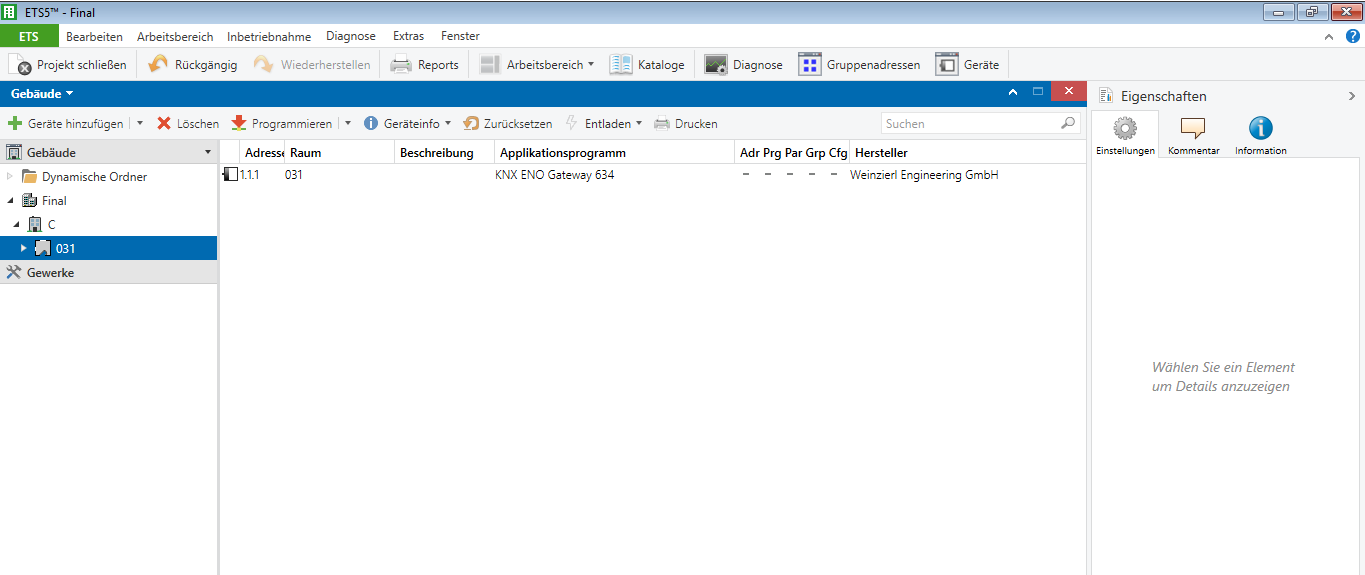
\includegraphics[width=13cm]{Doku/5}
	\caption{Übersicht der hinzugefügten Geräte}
	\label{fig:5}
\end{figure}

Damit die Geräte untereinander kommunizieren können müssen Gruppenadressen angelegt werden. Diese sind wie Geräte in einer dreistufigen Hierarchie angelegt. In den Abbildungen \ref{fig:6}, \ref{fig:7} und \ref{fig:8} kann betrachtet werden wie dies aussieht.

\begin{figure}[H]
	\centering
	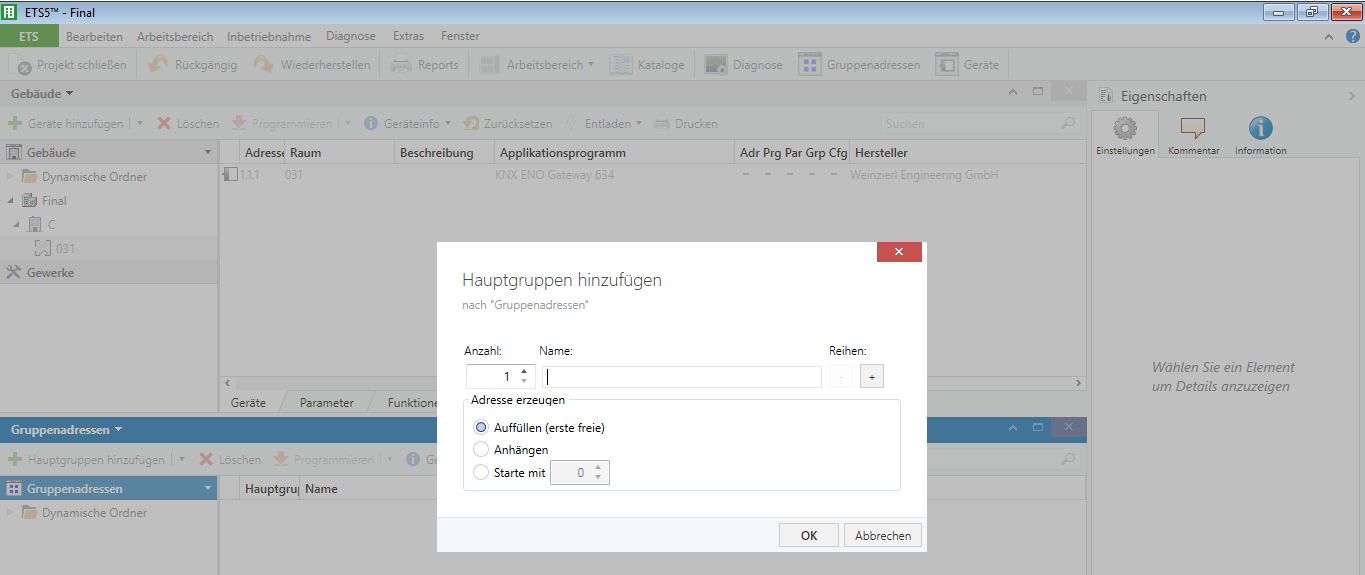
\includegraphics[width=13cm]{Doku/6n}
	\caption{Anlegen einer Hauptgruppe}
	\label{fig:6}
\end{figure}

\begin{figure}[H]
	\centering
	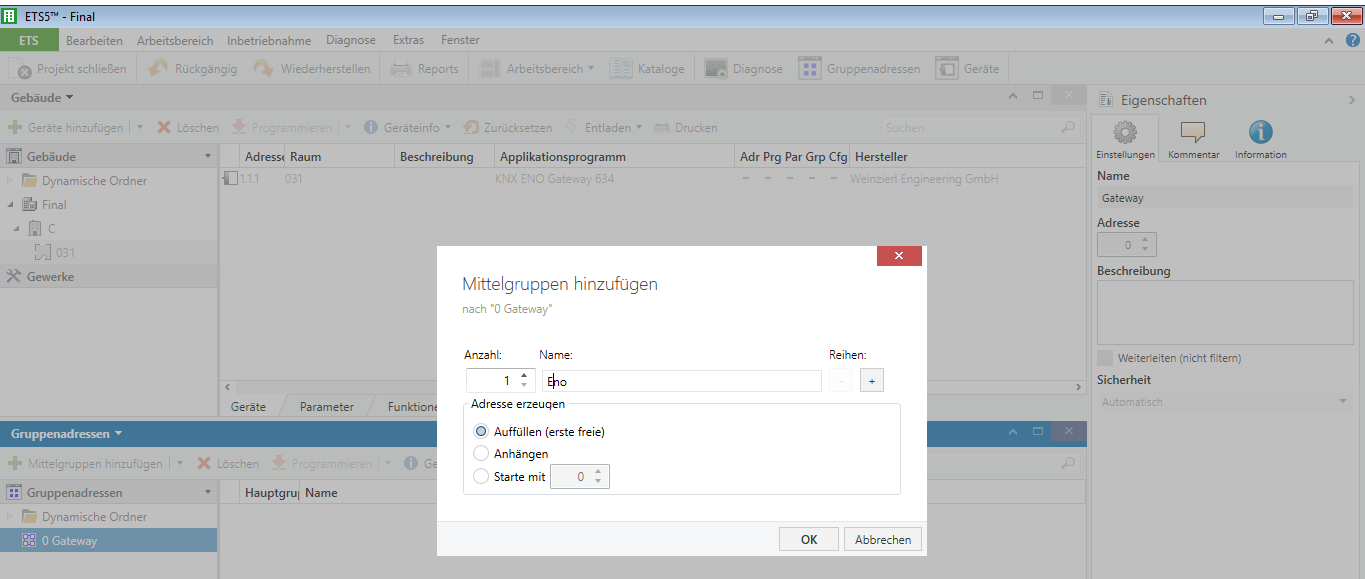
\includegraphics[width=13cm]{Doku/7n}
	\caption{Erstellen einer Mittelgruppe}
	\label{fig:7}
\end{figure}

\begin{figure}[H]
	\centering
	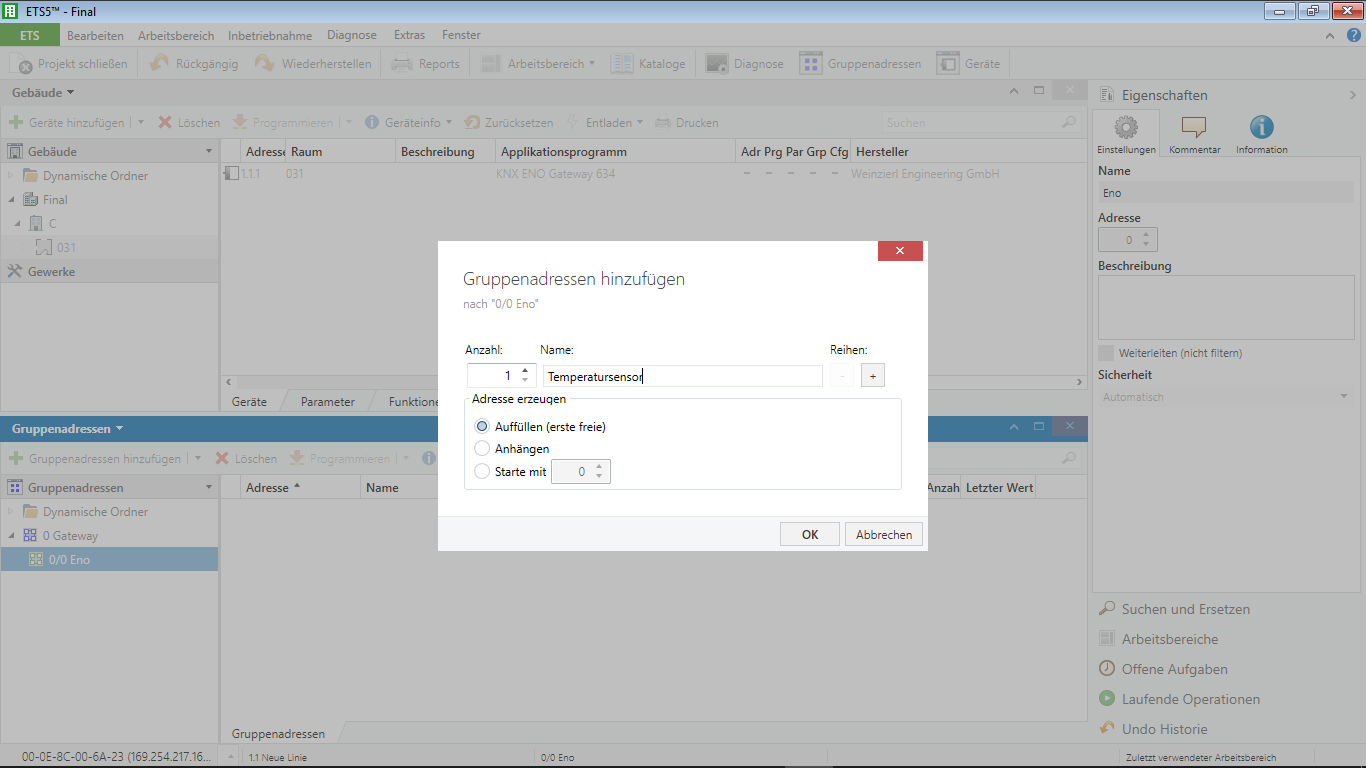
\includegraphics[width=13cm]{Doku/8}
	\caption{Gruppenadresse anlegen}
	\label{fig:8}
\end{figure}

\subsection{Konfiguration}
Zu erst muss die in KNX angelegte physikalische Adresse dem jeweiligen Gerät verknüpft werden. Dazu muss an dem Gerät der Programmierknopf gedrückt werden. Daraufhin leuchtet an dem Gerät eine rote LED. In ETS wählt man dazu unter \emph{Programmieren} die Option \emph{Physikalische Adresse} aus. Der Vorgang kann einige Sekunden dauern. Zusätzlich muss man sichergehen, dass eine Verbindung per TwistedPair oder ähnlicher KNX-Technologie zu der Hardware besteht.

Als nächstes muss das Gerät konfiguriert werden. In diesem Fall wurde das KNX ENO Gateway 634 auf Kanal 2 als EnOcean Aktor mit Antrieb für Stellventil A5-20-01 definiert. Siehe dazu Abbildung \ref{fig:11}

\begin{figure}[H]
	\centering
	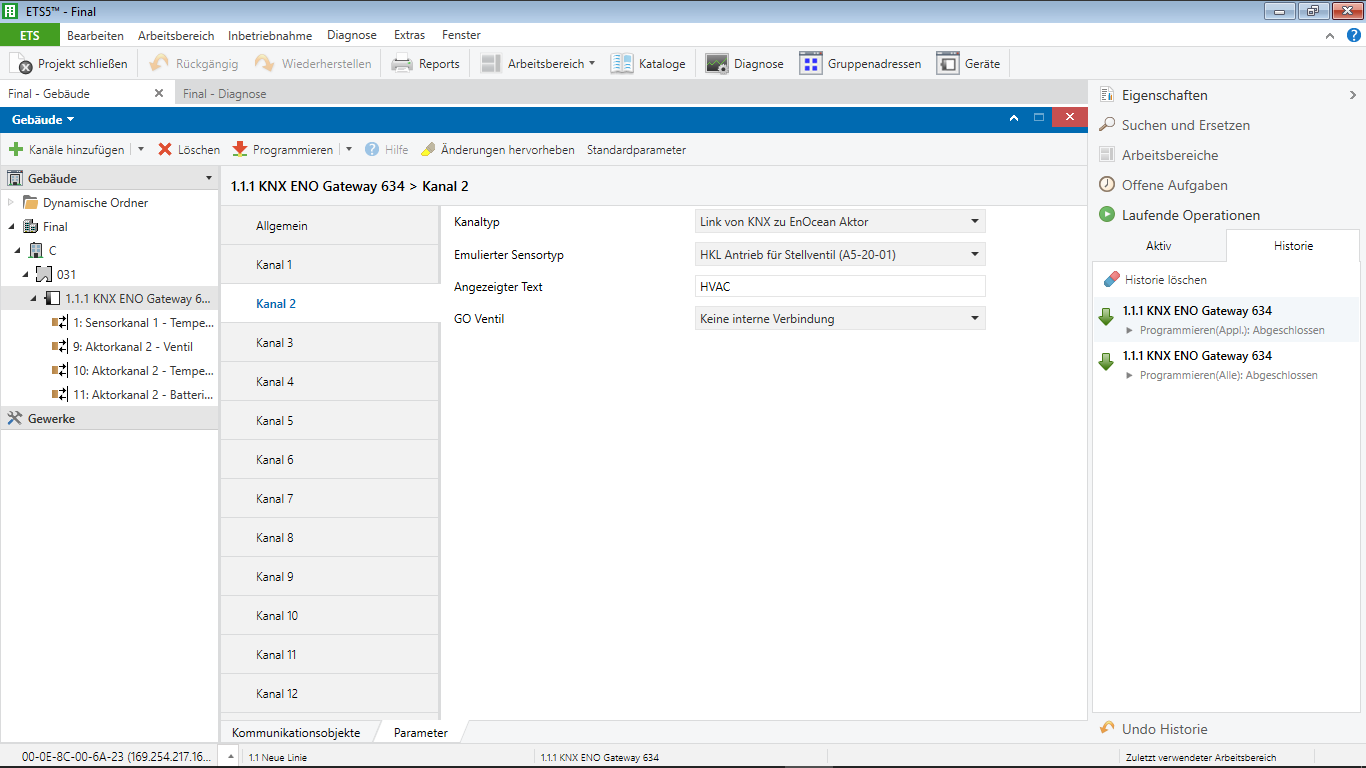
\includegraphics[width=13cm]{Doku/11}
	\caption{Konfiguration des KNX ENO Gateways}
	\label{fig:11}
\end{figure}

Damit eine Kommunikation zwischen Stellventil und Gateway möglich ist, muss am Gateway mit der Rechten Taste ein freier Kanal ausgewählt werden. Dann muss die rechte Taste länger gedrückt werden, bis eine Bildschirmänderung stattfand. An dem Stellventil muss daraufhin der Taster kurz gedrückt werden. Danach können die beiden Geräte miteinander kommunizieren. Es sei darauf zu achten, dass die Geräte beim Einlernen in Kommunikationsreichweite sind (maximal 300 Meter, praktisch eher 5 Meter)

Damit eine schnelle Debug-Kommunikation realisiert werden kann, muss das Stellventil so konfiguriert werden, dass es alle 2 Minuten Temperaturwerte an das Gateway sendet.
Dazu muss der Knopf an dem Stellventil so lange gedrückt werden bis die LED 4 mal grün und ein mal orange leuchtet. Dann muss der Taster erneut gedrückt werden bis die LED ein mal blinkt.

Zudem sollte die Energiesperre/Sommermodus deaktiviert werden. Dazu muss der Taster gedrückt werden bis die LED 4 mal grün leuchtet. Leuchtet die LED danach 2 mal grün muss ein mal der Taster betätigt werden.

Abbildung \ref{fig:12} zeigt die zyklische Temperaturmessung des Thermostats und übermittlung des gemessenen Wertes über EnOcean und KNX an den Busmonitor.

\begin{figure}[H]
	\centering
	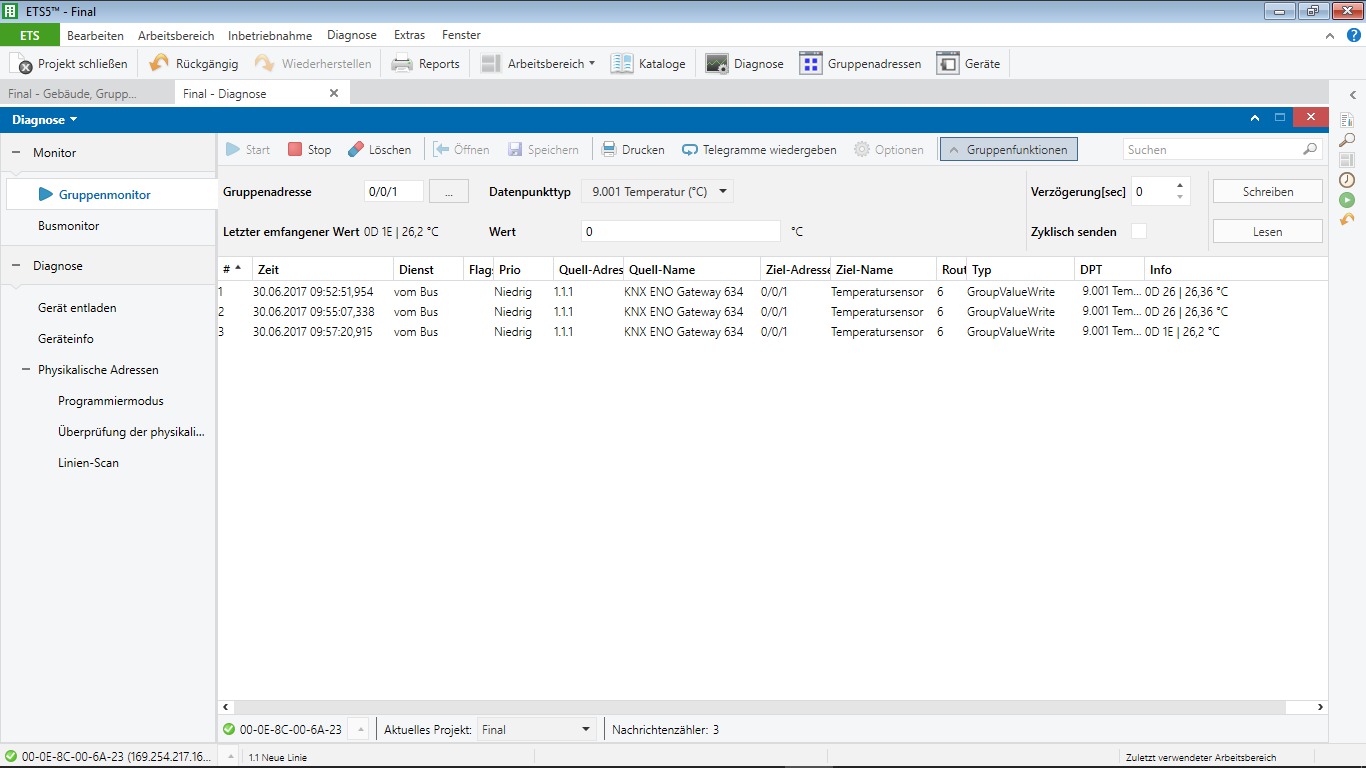
\includegraphics[width=13cm]{Doku/12}
	\caption{Konfiguration des KNX ENO Gateways}
	\label{fig:12}
\end{figure}

Es sei zu beachten, dass wenn man über den Busmonitor Werte Lesen und Schreiben möchte, die entsprechenden Berechtigungen gesetzt sein müssen. Wie in Abbildung \ref{fig:14} und \ref{fig:15} zu sehen ist, wurden dem Temperatursensor nur Leserechte gegeben während dem Ventil zusätzlich noch Schreibrechte gewährt wurden um den Wert manuell zu setzen.

\begin{figure}[H]
	\centering
	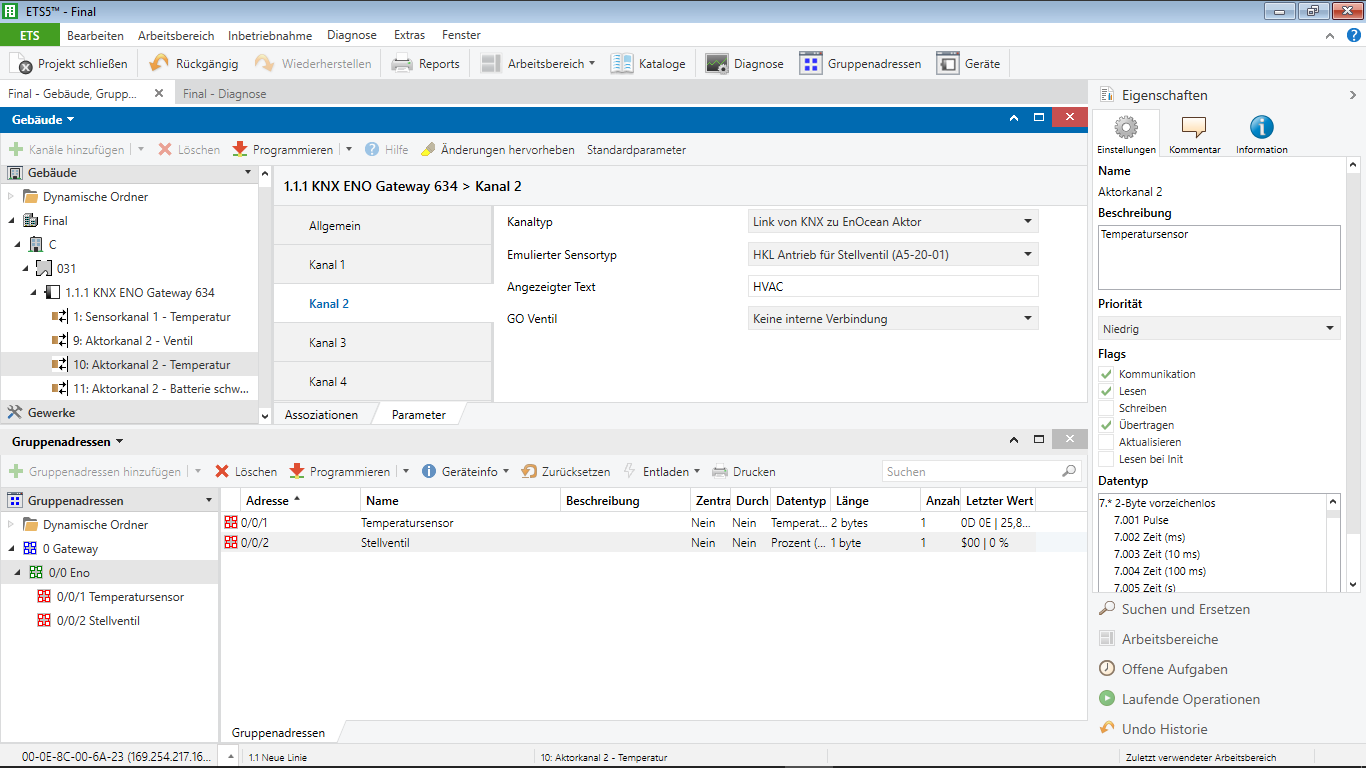
\includegraphics[width=13cm]{Doku/14}
	\caption{Rechte des Temperatursensors}
	\label{fig:14}
\end{figure}

\begin{figure}[H]
	\centering
	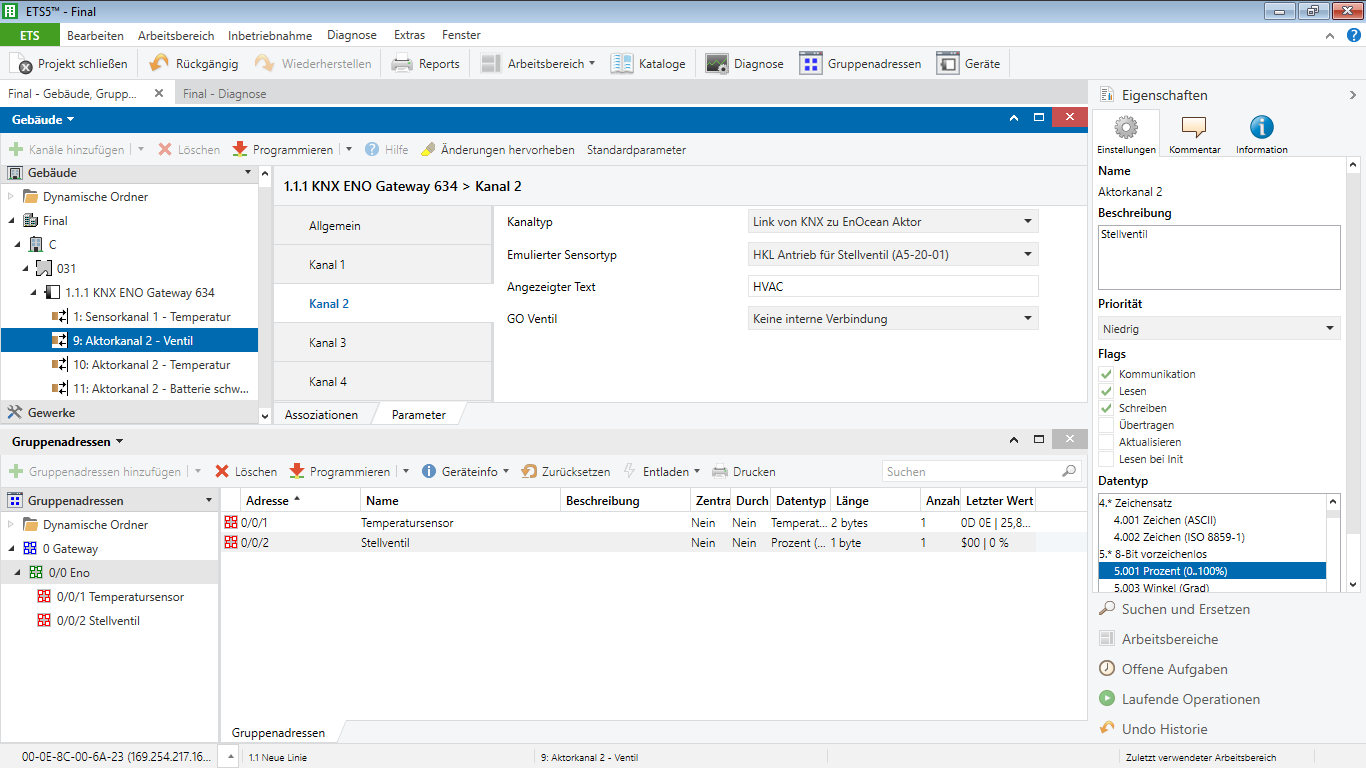
\includegraphics[width=13cm]{Doku/15}
	\caption{Rechte des Ventils}
	\label{fig:15}
\end{figure}

Um das Thermostat in einem Regelbetrieb automatisch zu betreiben wurde eine Regel angegeben um die Temperatur zu regeln. Wie in Abbildung \ref{fig:16} zu sehen ist, wurde der Sollwert der Temperatur zu Testzwecken auf warme 30 $^{\circ}$C gesetzt.

\begin{figure}[H]
	\centering
	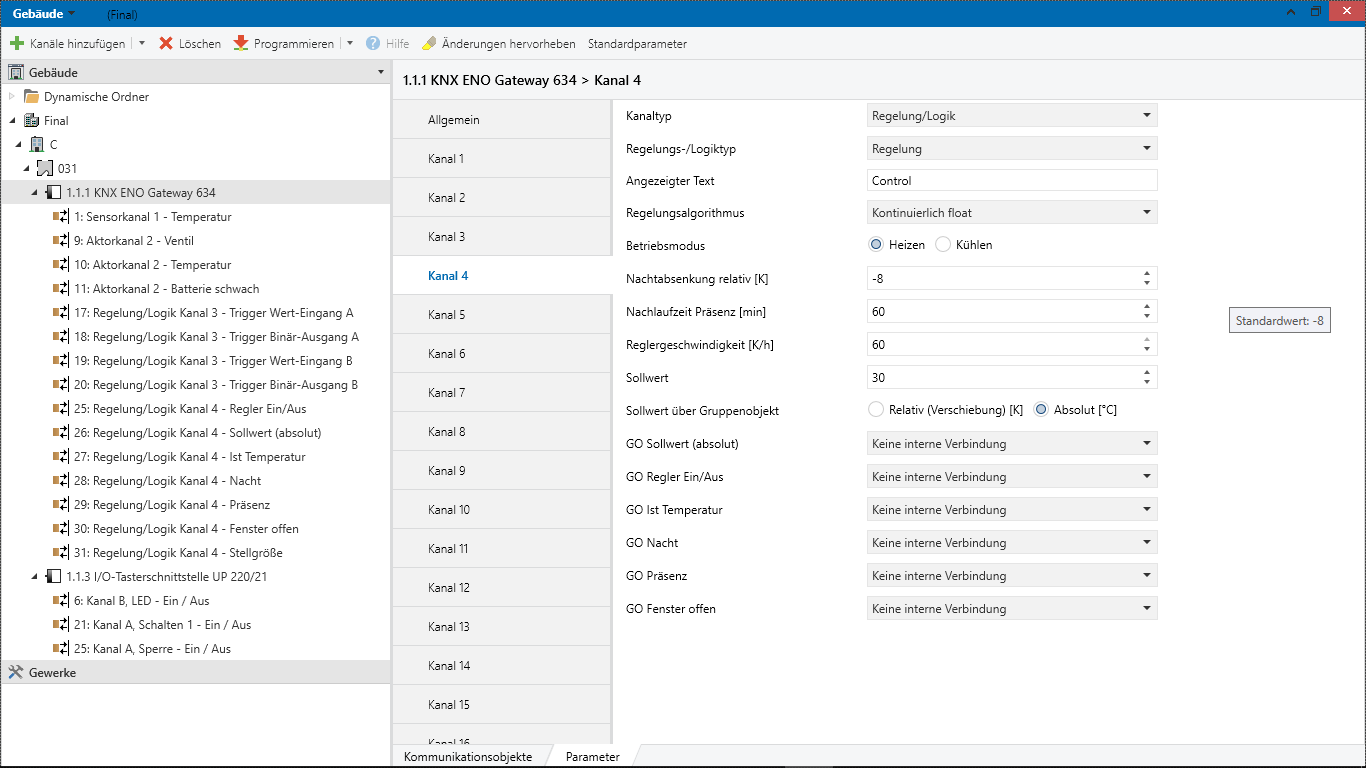
\includegraphics[width=13cm]{Doku/16}
	\caption{Regel zur Temperatursteuerung}
	\label{fig:16}
\end{figure}

Wie zuvor bereits erwähnt müssen die einzelnen Komponenten über Gruppenadressen miteinander verbunden sein um miteinander kommunizieren zu können.
Eine Übersicht über alle Gruppenadressen und deren Verknüpfung mit den jeweiligen Komponenten ist in den Abbildungen \ref{fig:17}, \ref{fig:18} und \ref{fig:19} zu finden.

\begin{figure}[H]
	\centering
	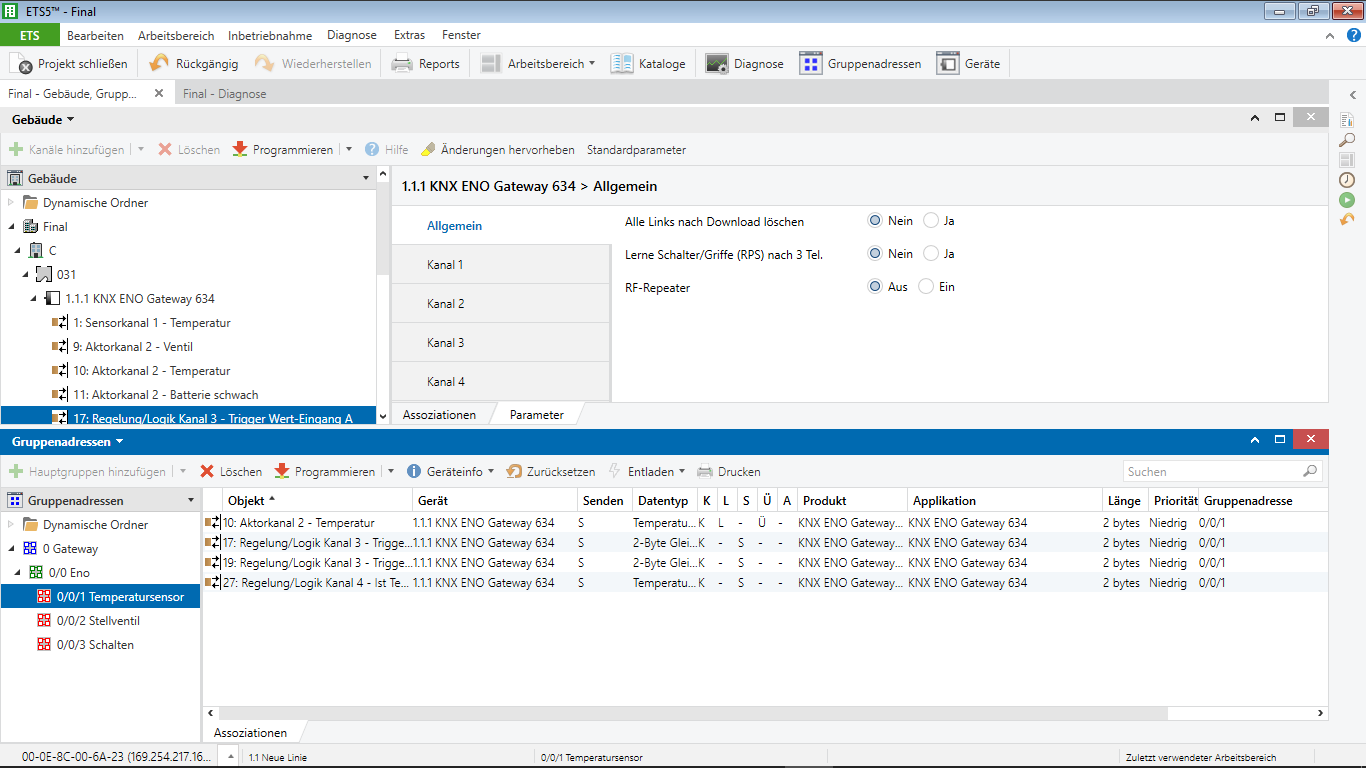
\includegraphics[width=13cm]{Doku/17}
	\caption{Gruppenadresse des Temperatursensors}
	\label{fig:17}
\end{figure}

\begin{figure}[H]
	\centering
	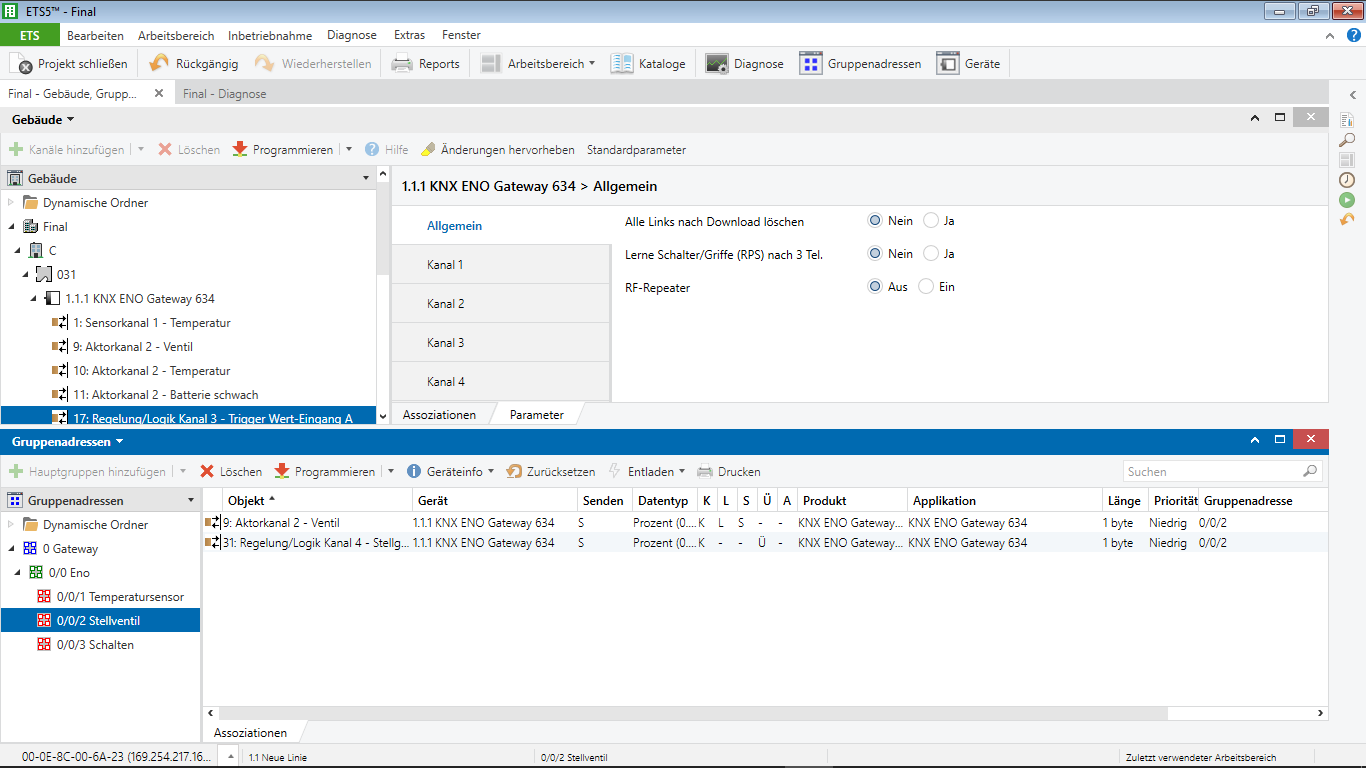
\includegraphics[width=13cm]{Doku/18}
	\caption{Gruppenadresse des Stellventils}
	\label{fig:18}
\end{figure}

Abschließend muss die Konfiguration auf die Hardware übertragen werden. Dazu wird in ETS unter \emph{Programmieren} die Option \emph{Applikationsprogramm} ausgewählt. Ein Drücken der Programmiertasten auf den Geräten ist nicht notwendig.

\subsection{Optional}
Außerdem wurde die auf dem Demoboard vorhandene IO-Tasterschnittstelle mitsamt Taster und LED benutzt. Diese wurde so konfiguriert, dass die Regelung so lange aktiv ist, bis der Taster gehalten wird.
Ein Leuchten der LED zeigt an, dass die Temperaturregelung aktiv ist.

Wäre ein KNX-fähiges Potentiometer verfügbar gewesen hätte man die Temperaturregelung noch variabel und damit praktisch einsetzbar machen können.
Da dies nicht der Fall war, wurde die Temperaturregelung in ETS auf 30 $^{\circ}$C fest eingestellt um die Funktionalität zu demonstrieren. Je nach Außentemperatur muss dieser Wert gegebenenfalls geändert werden.

\begin{figure}[H]
	\centering
	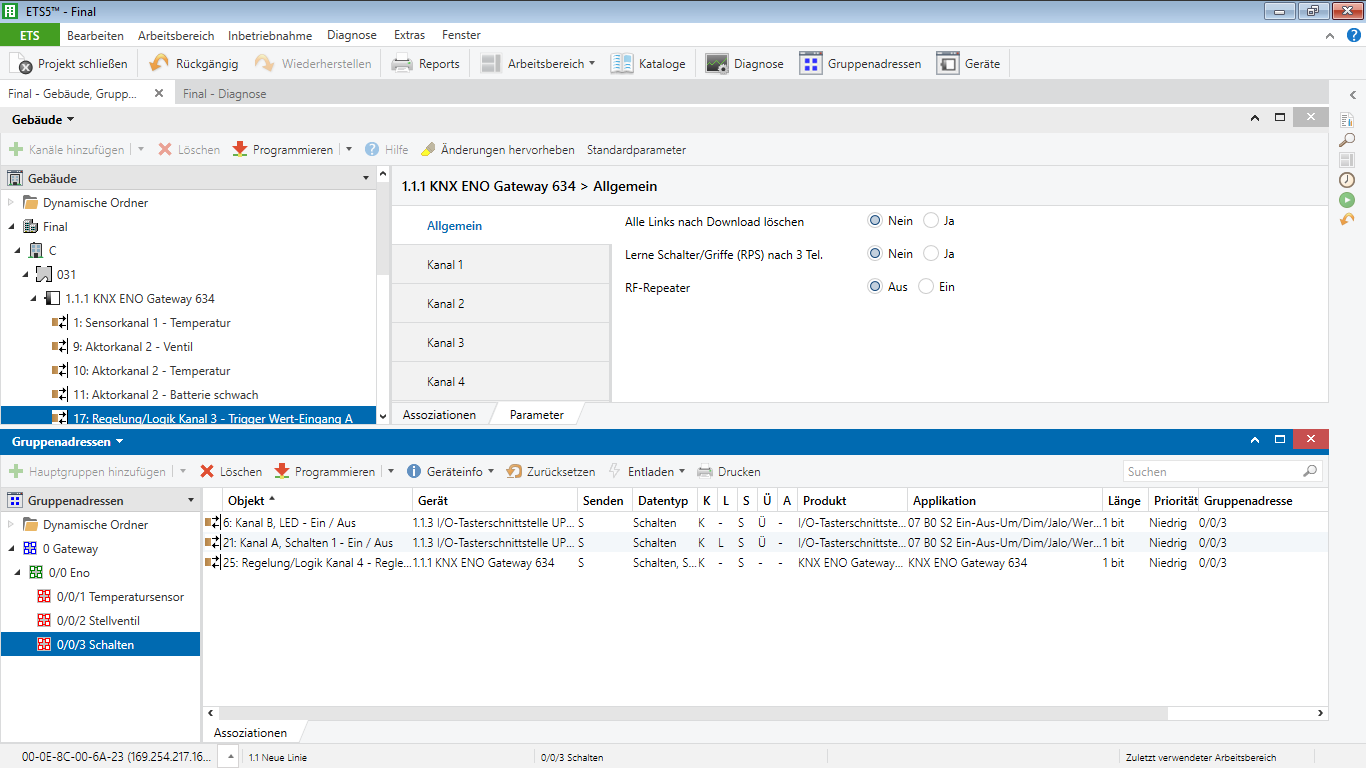
\includegraphics[width=13cm]{Doku/19}
	\caption{Gruppenadresse des Tasters}
	\label{fig:19}
\end{figure}
\section{Fazit}
Die Dokumentation des Stellventils ist teilweise fehlerhaft:
\begin{quotation}
	Wird der Taster solange gedrückt bis „sechs“ aufeinander folgende Signaltöne zu hören sind und die Status-LED „6x grün“ leuchtete, wird das Ende der Einstellungen durch „ein rotes“ Aufleuchten der Status-LED und einen langen Signalton ca. 1 s signalisiert.
\end{quotation}
Dies ist nicht richtig, da die LED leuchtet wie an anderer Stelle angegeben 4 mal grün, 1 mal orange und abschließend 1 mal rot.\\
\\
Zudem ist in der Dokumentation nirgends dokumentiert, dass das Gerät zuerst von sich aus mit KNX kommunizieren muss um danach auf lese/schreib-Kommandos zu reagieren. Andernfalls geschieht nichts. Dies dauert initial etwa 2 Minuten.\\
\\
Insgesamt hätte die Dokumentation besser sein können, in der öfters auf \emph{GO} eingegangen wurde, dies jedoch nirgends definiert wurde.\\
\\
Über Google konnten auch keine signifikante Hilfestellungen zur Konfiguration des Stellventils und dessen Funktionsweise gefunden werden.\\

\end{document}